\chapter{Data Acquisition and Software%
  \label{chap:\currfilebase}}

\section{Data acquistion}

The \ac{DAC} system developed in this thesis is an open source Arduino based system consisting of multiple microcontrollers. All signal channels are transmitted to a central microcontroller before passing to a computer that serves as visualization and analysis tool.

\begin{figure}[!htb]
  \centering
  \subcaptionbox{Without signal conditioning\label{sfig:dac_comp_simple}}
    {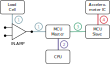
\includegraphics[scale=0.5]{figures/dac/dac_components/dac_comp_simple}}
    \hfill
  \subcaptionbox{With signal conditioning and external \ac{ADC}\label{sfig:dac_comp_precond}}
    {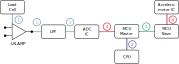
\includegraphics[scale=0.5]{figures/dac/dac_components/dac_comp_precond}}
  \\[0.5em]
  \caption[DAC building blocks]{\acs{DAC}-system building blocks --- note that~\ref{sfig:dac_comp_simple} has been realized, but~\ref{sfig:dac_comp_precond} has not been implemented yet, due to communication issues between the devices%
    \label{fig:dac_building_blocks}}
\end{figure}

\begin{table}[!htb]
  \centering
  \def\linelabel#1#2{%
    \begin{tikzpicture}[%
      x=1em,y=1ex,
      baseline=(N.south),
      font={\fontsize{6pt}{6.2pt}\selectfont},
      ]%
      \draw[#1, line width=1pt] (0,1) -- (1,1) node [
        midway, above, yshift=1,
        circle, fill=white, draw=#1, line width=1pt,
        inner sep=2pt, minimum size=8pt, align=center,
        ] (N) {#2};
  \end{tikzpicture}
  }
  \footnotesize
  \begin{tabular}{c@{:\hskip 0.5em}l}
    \toprule
    \multicolumn{2}{c}{Interfaces}\\
    \midrule
    \linelabel{WesMixL8qual0}{1} & Analog Signal\\
    \linelabel{WesMixL8qual3}{2} & \ac{USB}\\
    \linelabel{WesMixL8qual4}{3} & \ac{RS}-485\\
    \linelabel{WesMixL8qual6}{4} & \ac{SPI}\\
    \bottomrule
  \end{tabular}
  \normalsize
  \caption[Legend to DAC building blocks]{Legend to \figref{fig:dac_building_blocks}}
\end{table}

\subsection{Building Blocks}

Building blocks are the main components used in the \ac{DAC} signal chain. Additional components that are required to enable the stable operation of the building blocks are not listed.

Because the of accelerometer \ac{IC} output interfaces it is not possible to connect all sensors directly to one \ac{MCU} that acts as a \ac{DAC}. We need to transform the signal to a different interface. A low-cost and versatile method to achieve this, is to use a \ac{MCU} for each accelerometer \ac{IC}. These read the sensor \ac{IC} registers and communicate to the \ac{MCU} master. The master, on the other hand, acts as a passthrough and transmits the data to the \ac{CPU}. In the setup used, it also reads out the \ac{LC} signal. \tabref{tab:mcu_used} lists the \ac{MCU}s used during this thesis.% Other components can be found in \autoref{apx:appendix}.

The analog signal output of the \ac{LC} needs to be amplified to match the input range of the \ac{ADC}. To gain the maximum resolution, this depends on the expected input range. To get a higher value resolution than offered by the \ac{MCU} embedded \ac{ADC} one can set in an external \ac{ADC} \ac{IC} upstream to the \ac{MCU}. Additionally, we use a \ac{LPF} in \figref{sfig:dac_comp_precond}. The \ac{LPF} is needed to cut off high frequency components of the signal that occur particularly in sharp impulse signals. This design choice may lead to problems because it is not standard procedure in the development a measurement instrument. Typically, components in the analog signal chain are chosen, based on the frequency bandwidth of the input signal. This means, the cut-off frequency of the \ac{LPF} is set well above the signal's bandwidth. But because we use low-cost components in our system, the bandwidth is limited to half the sampling rate of the slowest sensor. According to the Nyquist frequency theorem, the cut-off frequency then needs to be reduced to half the sampling frequency, potentially reducing the output magnitude of higher frequency components of the signal.

\begin{table}[!htb]
  \centering
  \def\coltitle#1{\multicolumn{1}{c}{#1}}
  {\renewcommand{\arraystretch}{2.5}%
  \footnotesize
  \begin{tabular}{lcccccc}
    \toprule
    \coltitle{Name} &
    \coltitle{Core} &
    \coltitle{\makecell{\ac{ADC}-Reso-\\lution / \si{bit}}} &
    \coltitle{\makecell{Operating\\Voltage / \si{\volt}}} &
    \coltitle{\makecell{Clock Speed\\ / \si{\mega\hertz}}} &
    \coltitle{\makecell{Flash Me-\\mory / \si{\kilo Byte}}} &
    \coltitle{\makecell{SRAM\\ / \si{\kilo~Byte}}}\\
    \midrule
    Arduino Due & \makecell{AT91SAM3\\ARM Cortex} & 12 & 3.3 & 84 & 512 & 96\\
    Teensy 3.2 & \makecell{MK20DX256VLH\\Cortex-M4} & \makecell{13\\ \scriptsize{(\SI{16}{bit}-values)}} & 3.3 & 72 & 256 & 64\\
    \makecell[l]{Robotdyn\\Blackpill} & \makecell{STM32F103C8\\Cortex-M3} & 12 & 72 & 64 & 20\\
    \bottomrule
  \end{tabular}
  \normalsize
  }
  \caption[MCUs used]{List of \ac{MCU}s used in this work%
    \label{tab:mcu_used}}
\end{table}

Instrumental-Amplifier
AD627BRZ

Lowpass Filter
LTC1069-1IS8, 8th order, monolithic, clock tunable
LTC1154CN, highly customizable filter block
LTC1066-1, 8th order, clock tunable DAC

ADC
EVAL-AD7988, evaluation board for SAR-ADC





\subsection{Interfaces}

The interfaces are the connections and protocols between the different building blocks of the \ac{DAC} system. The interfaces are chosen based on the sensors used and the expected data rate at the required cable length between each section. I.e.:

\begin{itemize}
  \item Between the analog \ac{LC} and the external \ac{ADC} in \figref{sfig:dac_comp_precond} and the \ac{MCU} integrated \ac{ADC}  in \figref{sfig:dac_comp_simple} respectively the signal transmission is analog.
  \item The register of the accelerometer \ac{IC} is accessed via \ac{SPI}
  \item The communication between \acs{MCU}s is rooted in \acs{RS}-485 differential transmission to accommodate for signal transmission over cable lengths greater than \SI{10}{\meter} and uses a specialized protocol to keep data packages as small as possible.
  \item Between the \ac{MCU} and the \ac{CPU} \ac{USB} transmits data using the serial class of the Arduino software.
\end{itemize}

Data rates and package sizes are critical when sampling at high frequencies.

With \ac{RS}-485 data can be transmitted over distances of no less than \SI{100}{\km} at a data rate of \SI{1}{\kilo bit\per\second}. At \SI{1200}{\meter} cable length we can reach data rates of around \SI{100}{\kilo bit\per\second}. In our range of application, i.e.\ a few tens of \si{\meter}, we can expect data rates of \SI{1}{\mega bit\per\second}, thus representing the bottle neck in the digital data chain. If we then transmit \SI{80}{bit} acceleration measurements (see \figref{fig:data_flow}) at \SI{1.6}{\kilo\hertz} we stay below this expected limit by a safety factor of more than 10.
The arduino the serial package parses all data as human readable code, specifically \acf{ASCII}. In this format every digit of integer values is passed as \SI{8}{bit}-value. Which means that a \SI{32}{bit} timestamp and every single axis acceleration are passed as ten \SI{8}{bit}-values and six \SI{8}{bit}-values respectively. This increases the size of an accelerometer package to \SI{624}{bit}, which in turn reduces the safety factor to approximately 1.
It is clear that one cannot use human readable code to transmit the data and guarantee stability at the required sampling rate.


\subsubsection{MCU communication protocol}

The communication protocol for \ac{MCU} to \ac{MCU} and \ac{MCU} to computer was developed for this project.

\begin{table}[!htb]
  \centering
  \includestandalone[scale=1]{figures/software/mcu_com_protocol/mcu_com_protocol}
  \\[0.5em]
  \footnotesize
  \begin{tabular}{c@{:\hskip 0.5em}l}
    \toprule
    \large{\textcolor{WesMixL8qual6}{<[}/\textcolor{WesMixL8qual6}{]>}} & Start-/End-bytes, represented as \ac{ASCII}\\
    \textcolor{WesMixL8qual0}{\large (reg)} & Registry/Address of the transmission\\
    \textcolor{WesMixL8qual4}{\large (\#Bytes)} & Number of bytes in transmission\\
    \textcolor{WesMixL8qual5}{\large (data)} & Data to transmit\\
    \bottomrule
  \end{tabular}
\normalsize
  \caption[MCU communication protocol]{Protocol used to communicate between two MCU's and between MCU and computer%
    \label{tab:mcu_com_protocol}}
\end{table}

%     output signal that must be amplified by an \ac{IN-AMP} to scale up the signal to the operating range of the consecutive components.

% . to of smart sensor IC are predetermined. With \ac{SPI}Standard interfaces, determined by senor ic
% MCU com based uart length -> differential transmission using the rs-485 protocol, introduces slave master com, only one slave can speak at a time



\subsection{Dataflow}

The dataflow between the \ac{MCU}s is sequential and all data is passed to a central \ac{MCU}, called master, before we streamline it to the \ac{CPU}. The master cycles through all connected \ac{MCU} performing a data request, hold and receive action. As soon as a slave \ac{MCU} gets a request, it transmits a data package from its buffer. The master, now receiving the data package, will throughput the signal to the \ac{CPU}, where the data is stored. By the end of this process the master will jump to the next slave.

All measurements consist of a \SI{32}{bit}-timestamp and the measured values and are pushed into a \ac{FIFO} buffer in the flash memory of the \ac{MCU}, directly connected to the sensor. Bundled data packages are then pulled from the buffer and translated into the transmission code as defined in \tabref{tab:mcu_com_protocol}. In \figref{fig:data_flow} the data flow is represented by a system that is using only one slave \ac{MCU}, displayed in violet.

Clock synchronizations are executed in form digital data exchange, by synchronizing the timestamps before a complete measurement. The sensor measurements themselves are conducted as soon as ready to benefit of the sensors maximum measurement frequency. With this method, no data bandwidth is used between measurement cycles for clock synchronization, but it comes with three caveats. Firstly, every \ac{MCU} runs on its own clock cycle. Measurements are conducted whenever the individual time interval after the clock is exceeded. These time intervals are matched by sharing the master timestamp with the ones of the slave programmically. The slave timestamps are then tuned to same value during a setup process. But after the synchronization the Gausssian distributed deviations to the intervals accumulate, ultimately yielding unknown time-shifts to the signals.

Measurements are packaged due to the time the master requires to change the communication to another slave. During these switches no data is transmitted eventually limiting the data rate of the system.

\begin{figure}[!htb]
  \centering
  \includestandalone[width=0.8\linewidth]{figures/software/data_flow/data_flow}
  \caption[Data flow]{Data flow between two \ac{MCU}s and the CPU%
    \label{fig:data_flow}}
\end{figure}

\section{Software}

The software developed during this project is split into the Arduino software running on the \acs{MCU}s and a python based tool to receive and visualize the data via \ac{USB}.

For the instrument to work, some functions are required, while other desired functions are tools that simplify the workflow during measurements and facilitate bug fixes in the software.

The requirements to the software tools are:
\begin{enumerate}
  \item Read out accelerometer and \ac{LC} data at the maximum sample speed of the accelerometer \ac{IC}.\label{req:read_out}
  \item Synchronize measurements timestamps.\label{req:sync}
  \item Initialize measurement by hammer impulse.\label{req:init}
\end{enumerate}

The desired software tools are:
\begin{enumerate}[resume]
  \item Generate continuous real time output of measurement data.\label{des:cont_out}
  \item Track data transfer via \ac{USB}.\label{des:dat_track}
\end{enumerate}

\subsection{Implementation}

For data communication, all data software used in this project use a standardized input and output of the package format described in \tabref{tab:mcu_com_protocol}; where the addresses are used as identifiers.

\subsubsection{Common Addresses}
Addresses are identified by a parser that identifies the instruction contained in the address. Every device is assigned to handle predefined addresses accordingly. That is, it processes the instruction or it transmits the data package to then next device. Every data package keeps its address as defined in \tabref{tab:mcu_com_protocol} from start to destination. A measurement package, for example includes multiple measurements in the data block and has an address specific to the measurement sensor, with its destination to the \ac{CPU}, whereas a command from the computer application has a destination address to one specific \ac{MCU}; all \ac{MCU}s inbetween the two devices transmit the data as is. For this reason, although the parser is defined by the same class in every device, it requires an additional identification to detect on which device the parser is running.

\subsubsection{Microcontroller Software}
The software running on the \ac{MCU} is programmed in the Arduino programming language and uploaded via bootloader. This way, the software can be uploaded by a serial interface but, additionally to the software itself, some of the flash memory is reserved for the bootloader. The remaining memory is used during operation is used for a digital \ac{FIFO} buffer.
Because all used \ac{MCU}s are using one core only, parallel data transfer is not possible and the data must be merged and serialized at the master \ac{MCU}. Both the parser and the buffer add an overhead to the cyclic running program on the \ac{MCU} that potentially limits the communication speed.

\subsubsection{Computer Software}
The software on the computer runs in python. As a key module that enables the communication between the running python script and the serial port the pyserial has been used. The software tools are able to identify, store and visualize the captured data.

\subsection{Challenges}

\subsubsection{Time Synchronization}

The time synchronization between the \ac{MCU}s is handled on software level. The master sends its current clock as a data package to the slaves and they adapt their clocks accordingly. This can be conducted in multiple ways. TODO
